\chapter{Methodology}
This chapter summarizes the methodology used to develop the recovery system for this thesis.
In short, the recovery system is developed example-driven using the model of a fictional \gls{HRMS} used by the 101wiki\footnote{\url{https://101wiki.softlang.org/} (retrieved \formatdate{12}{11}{2017})} for its contributions.

\section{Example Driven Development Process}
The Example Driven Development Process used to develop the recovery system for this thesis is shown in Figure \ref{figure:ExampleDrivenDevelopment}.
\begin{figure}[h!]
\begin{center}
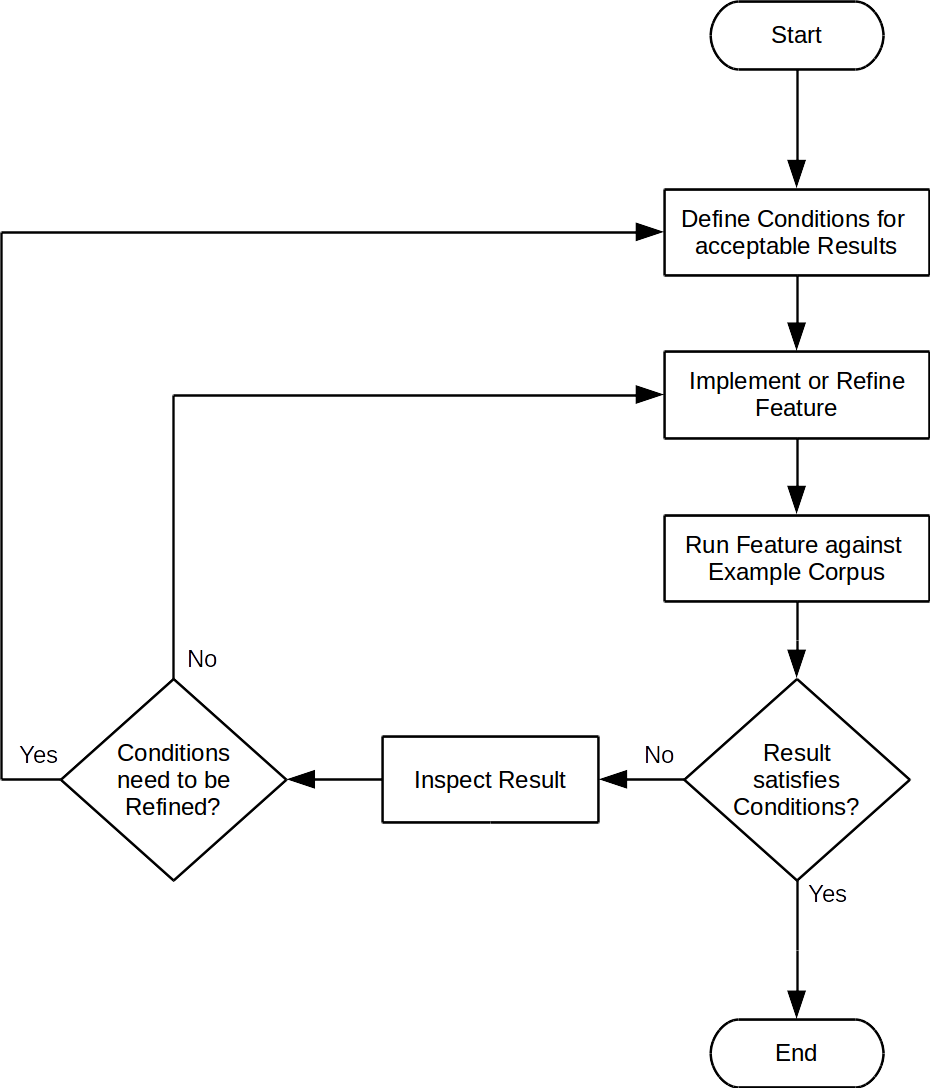
\includegraphics[scale=.4]{images/ExampleDrivenDevelopment.png}
\end{center}
\caption{The Example Driven Development Process}
\label{figure:ExampleDrivenDevelopment}
\end{figure}
Given we acquired a suitable example corpus, which is outlined in detail in §\ref{section:ExampleCorpus}, we have to define conditions for acceptable results.
These conditions can be seen as functional requirements, for instance, we want a \gls{Java} class artifact to be linked via correspondence to its \gls{XML}-serialized form:
{
\footnotesize
\begin{align*}
\texttt{public class Company \{...\}} \correspondsTo \texttt{<company>...</company>}
\end{align*}
}%
Then we implement a feature which produces the specified results and run it against the example corpus.
If the result meets all conditions we are done.
If not, we inspect the results to check whether our predefined conditions are to vague or wrong.
If so, we refine our conditions, if not, we refine our feature implementation
Either way the process starts anew.


\section{Example Corpus}
\label{section:ExampleCorpus}
The example corpus used to develop the recovery system for this thesis consists of artifacts implementing a fictional \gls{HRMS} within an \gls{O/R/X-Mapping} scenario using \gls{Java} technologies.
The model is implemented using plain \Gls{Java}. 
It is then mapped to plain \gls{XML}/\gls{XSD} with \gls{JAXB} and to \gls{SQL/DDL} statements using \gls{Hibernate} mapping files and/or annotations.



\subsection{The 101HRMS Model}
\gls{101HRMS}\footnote{\url{https://101wiki.softlang.org/101:@system} (retrieved \formatdate{12}{11}{2017})} provides a simple model of a company with many departments and employees.
Figure \ref{figure:101HRMSModel} shows an \gls{UML} class diagram of a variant of this model.

\begin{figure}[h!]
\begin{center}
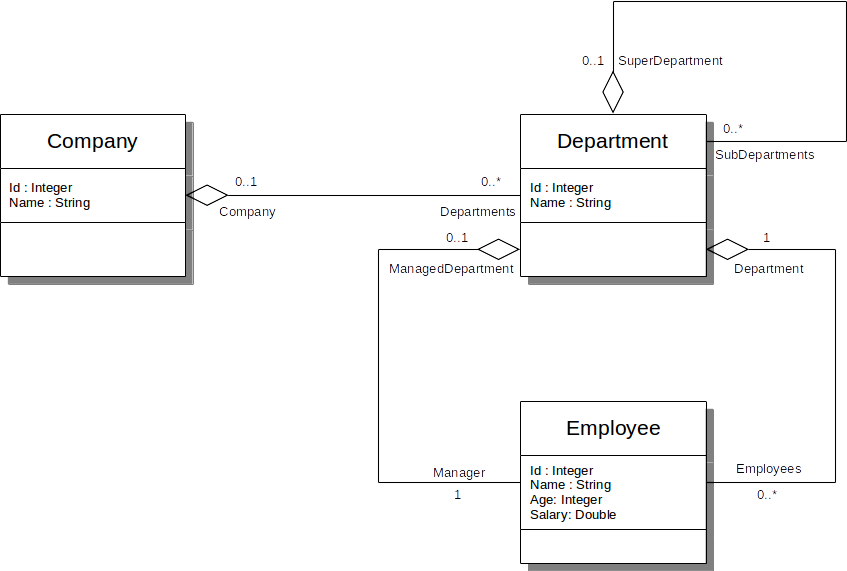
\includegraphics[scale=.5]{images/101HRMSModel.png}
\end{center}
{
\scriptsize 
This \gls{UML} class diagram depicts the model of the \gls{101HRMS}.
It consists of simple companies with nested departments and employees mapped to the latter.
}
\caption{The 101 Human Resource Management System Model}
\label{figure:101HRMSModel}
\end{figure}

The \gls{101HRMS} model consists of companies attributed with a name.
Each company accumulates departments.
Each department is also attributed with a name, aggregates employees and has one employee acting as manager.
Departments can further be refined into sub-departments.
Each employee is attributed with a name, an age and a salary.
Each entity is also attributed with an ID.

\subsection{Linguistic Domains of the Example Corpus}
The example corpus used to develop the recovery system contains artifacts implementing the \gls{101HRMS} model generated or used by \gls{Java} technologies for \gls{O/R/X-Mapping}, i.e. a \gls{Java} model is mapped to plain \gls{XML}/\gls{XSD} with \gls{JAXB}, to a \gls{Hibernate} mapping file and to \gls{SQL}/\gls{DDL} statements.
Figure \ref{figure:ExampleCorpusJORXDomains} shows a schematic illustration of the linguistic domains involved:
\begin{description}

\item[Java]
The language and technology used to implement the \gls{101HRMS} model.

\item[XML]
The language used to serialize the \gls{101HRMS} model.

\item[SQL/DDL]
The language used to persist the \gls{101HRMS} model.

\item[JAXB]
The technology used to implement \gls{O/X-Mapping} of the \gls{101HRMS} model.

\item[Hibernate]
The technology used to implement \gls{O/R-Mapping} of the \gls{101HRMS} model.

\end{description}

\begin{figure}[h!]
\begin{center}
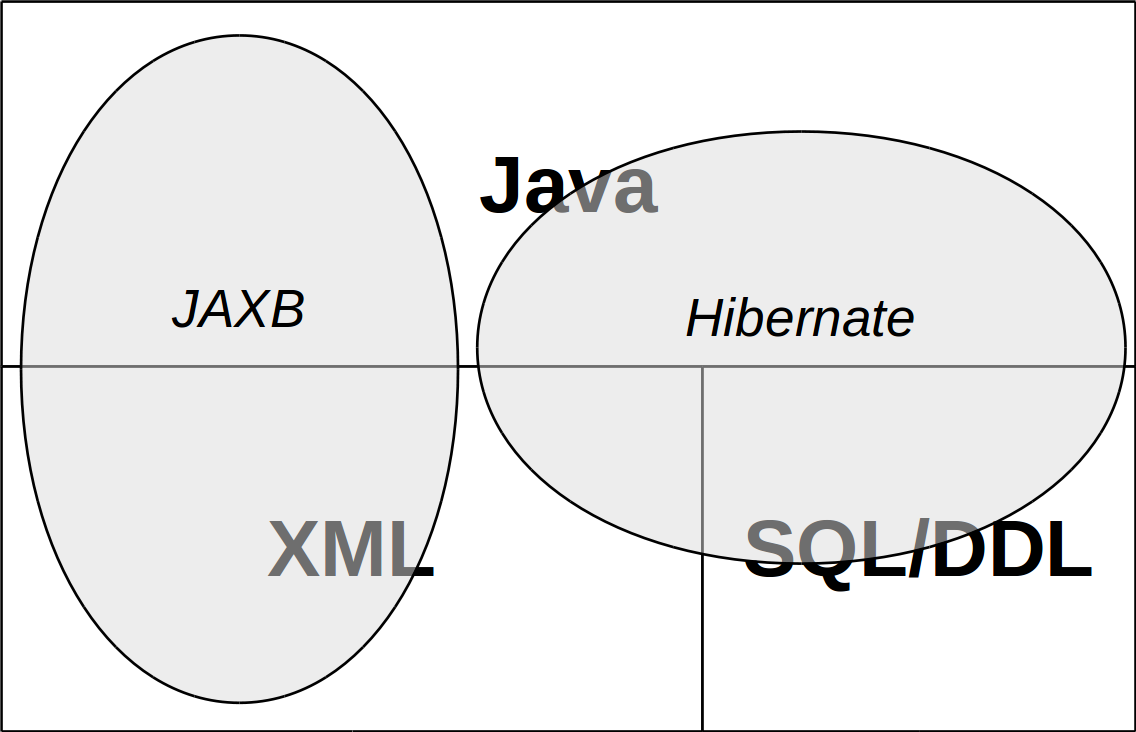
\includegraphics[width=.6\textwidth]{images/JORXDomains.png}
\end{center}
{
\scriptsize 
This schematic illustration depicts the interrelation among linguistic domains of example corpus used.
It depicts languages and technologies for \gls{O/R/X-Mapping} with \gls{Java}.
}
\caption{Example Corpus Domains: Java O/R/X}
\label{figure:ExampleCorpusJORXDomains}
\end{figure}

The languages (\gls{Java}, \gls{XML} \& \gls{SQL}) in Figure \ref{figure:ExampleCorpusJORXDomains} are displayed as disjoint square sets.
Technologies (\gls{JAXB} \& \gls{Hibernate}) are displayed as oval sets intersecting languages.
This is due to their linguistic nature, e.g. \gls{JAXB} produces specific \Gls{Java}- and \gls{XML}-Code which does not necessarily intersect with code produced by other technologies.
\gls{Hibernate} intersects all three languages.
It uses \gls{XML} files or \gls{Java}-Annotations for describing \gls{O/R-Mapping} of a data-model and generates \gls{SQL} artifacts according to that mapping.
In this sense, technologies create technology-specific subsets of a languages.


%\section{Link Proper Part Ratio}
%The ratio between all proper parts of two artifacts and the proper parts of the same artifacts in a relationship.
%
%\begin{align*}
%\pi_{R,A_1,A_2} = \frac{|\{ (p_1,p_2) \in R : p_1 \properPartOf A_1 \wedge p_2 \properPartOf A_2 \}|}{|\{ p : p \properPartOf A_1 \vee p \properPartOf A_2\}|}
%\end{align*}